%!TEX root = mainfile.tex

\subsection{Observational Gravitational Lensing} % (fold)
\label{sec:observational_gravitational_lensing}
	Gravitational lensing will enhance the observing capabilities of any telescope used allowing some of the most distant objects in the universe to be seen. Since one of the aims of this project is to push current boundaries and observe objects at as yet unexplored redshifts, lensing will prove to be a very useful tool. Lensed sources at redshifts above 7 tend to be magnified by a factor of 5 to 10 over an area of 1 square arcminute, however this magnification can be as much as 30 times for certain source locations\cite{magnification}. Two routes were considered to include gravitational lensing in the observing strategy: either new lenses could be located or lenses found by other surveys could be selected. This section lays out the properties desired for the lenses chosen and the arguments for each of these options.

	\subsubsection{Constraints on the Lenses} % (fold)
	\label{sub:constraints_on_the_lenses}
		The lenses used will be chosen depending on the suitability of their properties for the observing strategy. Firstly, the area of the sky in which the lenses lie must be chosen carefully, particularly if a ground based telescope is used. The region of sky must be chosen to be compatible with the direction in which the telescope(s) used for the deep survey are able to point. For a space based telescope, this is not a major issue since they are not confined by the Earth's motion. Any regions with bright foreground contaminants would be ruled out and the lenses would be chosen such that they are distributed across the sky in order to reduce the effect of cosmic variance. Another factor that must be accounted for is that the lensing cross section of an object is directly dependent on its mass, as shown in Figure~\ref{fig:Lensing_cross_section_as_a_function_of_mass}\cite{Optimal_mass_configurations}. This would suggest that the lenses chosen should be very massive and are therefore likely to be galaxy clusters.
		\begin{figure}[htbp]
			\centering
				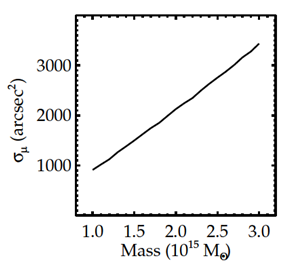
\includegraphics[width=0.4\textwidth]{../Images/Lensing_cross_section_as_a_function_of_mass.png}
			\caption[Lensing cross section as a function of mass]{\cite{Optimal_mass_configurations}Plot of the lensing cross section as a function of mass for a spherical halo at $z=0.5$. The dependence of cross section on mass can be clearly seen, indicating that the more massive a cluster, the better a lens it will be.\label{fig:Lensing_cross_section_as_a_function_of_mass}}
		\end{figure}

		The source magnification is also sensitively dependent on the lens redshift, though constraining this is less straightforward as there is a trade-off between Einstein angle and shear. On the one hand, the Einstein angle, an indicator of the strength of a lens, increases as the lens redshift decreases. Figure~\ref{fig:Einstein_angle_as_a_function_of_source_redshift} shows how lens redshift varies with Einstein angle. The point at which each curve crosses the x-axis is the lens redshift, since no lensing occurs when the source and lens redshifts are equal. For each value of lens redshift, the Einstein angle increases rapidly at source redshifts slightly greater than that of the lens, and then quickly saturates\cite{Constraining_source_redshift_distributions}. The lower the redshift of the lens, the higher the saturation value, suggesting lower lens redshifts are the best.
		\begin{figure}[htbp]
			\centering
				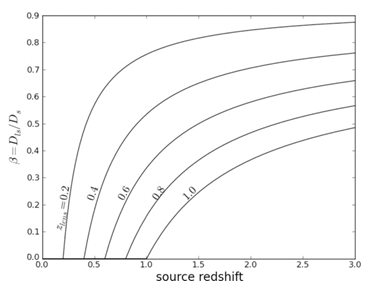
\includegraphics[width=0.5\textwidth]{../Images/Einstein_angle_as_a_function_of_source_redshift.png}
			\caption[Einstein angle as a function of source redshift]{\cite{Constraining_source_redshift_distributions} Plot of Einstein angle against source redshift. Again, each line corresponds to a different lens redshift. The point at which each line crosses the x-axis is the lens redshift, since at the lens, the magnification of the source is equal to 0.\label{fig:Einstein_angle_as_a_function_of_source_redshift}}
		\end{figure}

		However, the extent to which the images are distorted is not taken into account. The shear caused by a lens at a particular redshift is given by
		\begin{align}
			\gamma(r) &= \frac{4\pi G}{c^2}\frac{D_{LS}D_L}{D_S}\left( \overline{\Sigma}(<r)-\Sigma(r) \right)
		\end{align}
		where $\overline{\Sigma}(<r)$ is the mean projected surface mass density within r and $\Sigma(r)$ the projected surface mass density at $r$. Keeping the radius (and therefore surface mass density) constant, Figure~\ref{fig:shear_as_a_function_of_source_redshift} shows the dependence of shear on source redshift at the same fixed lens redshifts as the plot above. lens redshifts as the plot above. It can be seen from this plot, that at low source redshifts, the shear distortion is immeasurably small. As the redshift increases to around 0.5, the clusters at the lowest redshifts cause some significant distortion. Once the source redshift is greater than 1, shear distortion is seen around clusters at all the lens redshifts plotted\cite{Constraining_source_redshift_distributions}.
		\begin{figure}[htbp]
			\centering
				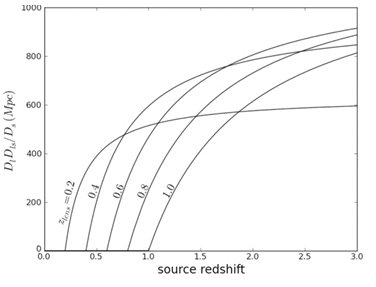
\includegraphics[width=0.5\textwidth]{../Images/Shear_as_a_function_of_source_redshift.png}
			\caption[Shear as a function of source redshift]{\cite{Constraining_source_redshift_distributions}A plot of shear against source redshift, with each line representing a different lens redshift. The point at which the lines cross the x-axis is the lens redshift, since at the lens, the magnification of the source is equal to 0.\label{fig:shear_as_a_function_of_source_redshift}}
		\end{figure}

		It has also been found that giant arcs are most likely to form behind higher redshift lenses, as shown in Figure~\ref{fig:Arc_probability}. Giant arcs are observed in systems where the shear is large. Lensing clusters at a redshift above 0.5 have been found to have an arc formation probability up to 3 times that of lower redshift lenses. Clusters observed at $z>0.5$ have also been found as a general rule to be less massive than closer clusters, indicating that clusters at this redshift are more efficient lenses. As a result, a judicious choice of lens redshift must be made to optimise both lensing strength and distortion for the best chance of observing high redshift galaxies\cite{wu_and_chiueh}.
		\begin{figure}[htbp]
			\centering
				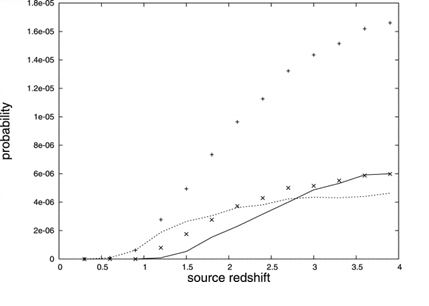
\includegraphics[width=0.5\textwidth]{../Images/Arc_probability.png}
			\caption[Arc probability]{\cite{wu_and_chiueh}Plot of the arc probability against source redshifts in four different lens intervals, $0.14\le z_L\le 0.45$ (dotted line), $0.49\le z_L\le 0.68$ (crosses), $0.73\le z_L\le 0.94$ (solid line), and $0.14\le z_L\le 0.94$ (plus signs).\label{fig:Arc_probability}}
		\end{figure}
	% subsection constraints_on_the_lenses (end)

	\subsubsection{Locating New Lenses} % (fold)
	\label{sub:locating_new_lenses}
		Locating new lenses would be advantageous in that the lenses could be chosen with the tight constraints specified above such that their properties are tailored to suit the needs of our strategy. The lenses would be selected using some form of wide survey by means of their strong lensing properties since objects that lense strongly are likely to be better for observing very faint sources. The parameters describing the lenses located would not be known so calculations to find these must be carried out. Taking the Einstein radius to be the average distance of the arcs from the centre of the lens, and assuming that most of the mass of the cluster is enclosed within this radius, an estimate of the mass can be found from
		\begin{align}
			M &= \Sigma_c\pi \theta_E^2 \label{eq:new_lens_mass_estimate}
		\end{align}
		The critical surface density, as defined in equation~(\ref{eq:new_lens_mass_estimate}) can be found when the source redshift is known and the magnification of the source can then be calculated as detailed in Section~\ref{sec:gravitational_lensing}.
	% subsection locating_new_lenses (end)

	\subsubsection{Using Known Lenses} % (fold)
	\label{sub:using_known_lenses}
		The second option, selecting known lenses has the advantage that the masses and velocity dispersions would already be well determined, allowing an accurate calculation of the magnification to be made. Examples of surveys that have been carried out previously include the Cluster Lens And Supernova survey with Hubble (CLASH)\cite{CLASH} and the MAssive Cluster Survey (MACS)\cite{MACS}. There are only a limited number of massive clusters known, however even with the small sample available, many interesting sources have already been observed for example a candidate $z\approx11$ galaxy behind cluster MACSJ0647.7+7015\cite{CLASH_z11_candidate}. Unless a wide survey is carried out as part of the observing strategy, using known lenses would significantly reduce the observing time required for the strategy compared to requiring an additional survey to locate new lenses. Both MACS and CLASH select their source using x-rays in order to obtain an unbiased distribution of masses, however, for this strategy the lenses would be chosen from these catalogues based on their masses and lensing properties.

	% subsection using_known_lenses (end)
% section observational_gravitational_lensing (end)
